\documentclass{article}
\usepackage[utf8]{inputenc}
\usepackage{comment}
\usepackage{graphicx}
\graphicspath{ {./pictures/} }
\usepackage{hyperref}
\usepackage{float}
\usepackage{listings}
\usepackage{algpseudocode}

% Kodierung, Sprache, Patches {{{
\usepackage[T1]{fontenc}    % Ausgabekodierung; ermöglicht Akzente und Umlaute
                            %  sowie korrekte Silbentrennung.
\usepackage[utf8]{inputenc} % Erlaubt die direkte Eingabe spezieller Zeichen;
                            %  utf8 muss die Eingabekodierung des Editors sein.
\usepackage[ngerman]{babel} % Deutsche Sprachanpassungen (z.B. Überschriften).
\usepackage{microtype}      % Optimale Randausrichtung und Skalierung.
\usepackage[
    autostyle,
    ]{csquotes}             % Korrekte Anführungszeichen in der Literaturliste.
%\usepackage{fixltx2e}      % Patches fuer LaTeX2e - seit 2015 nicht mehr nötig
\usepackage{scrhack}        % Verhindert Warnungen mit älteren Paketen.
\usepackage[
  newcommands
]{ragged2e}                 % Verbesserte \ragged...Befehle
\PassOptionsToPackage{
  hyphens
}{url}                      % Sorgt für URL-Umbrüche in Fußzeilen u. Literatur
% }}}

% Schriftarten {{{
\usepackage{mathptmx}       % Times; modifies the default serif and math fonts
\usepackage[scaled=.92]{helvet}% modifies the sans serif font
\usepackage{courier}        % modifies the monospace font
% }}}

% Biblatex {{{
\usepackage[
    style=alphabetic,
    backend=biber,
    %backref=true
    ]{biblatex}             % Biblatex mit alphabetischem Style und biber.
\bibliography{\jobname.bib} % Dateiname der bib-Datei.
\DeclareFieldFormat*{title}{
    \mkbibemph{#1}}         % Make titles italics
% }}}

% Dokument- und Texteinstellungen {{{
\usepackage[
    a4paper,
    margin=2.54cm,
    marginparwidth=2.0cm,
    footskip=1.0cm
    ]{geometry}             % Ersetzt 'a4wide'.
\clubpenalty=10000          % Keine Einzelzeile am Beginn eines Absatzes
                            %  (Schusterjungen).
\widowpenalty=10000         % Keine Einzelzeile am Ende eines Absatzes
\displaywidowpenalty=10000  %  (Hurenkinder).
\usepackage{floatrow}       % Zentriert alle Floats
\usepackage{ifdraft}        % Ermöglicht \ifoptionfinal{true}{false}
\pagestyle{plain}           % keine Kopfzeilen
% \sloppy                    % großzügige Formatierungsweise
\deffootnote{1em}{1em}{
  \thefootnotemark.\ }      % Verbessert Layout mehrzeiliger Fußnoten

\makeatletter
\AtBeginDocument{%
    \hypersetup{%
        pdftitle = {\@title},
        pdfauthor  = \@author,
    }
}
\makeatother
% }}}

% Weitere Pakete {{{
\usepackage{graphicx}       % Einfügen von Graphiken.
\usepackage{tabu}           % Einfügen von Tabellen.
\usepackage{multirow}       % Tabellenzeilen zusammenfassen.
\usepackage{multicol}       % Tabellenspalten zusammenfassen.
\usepackage{booktabs}       % Schönere Tabellen (\toprule\midrule\bottomrule).
\usepackage[nocut]{thmbox}  % Theorembox bspw. für Angreifermodell.
\usepackage{amsmath}        % Erweiterte Handhabung mathematischer Formeln.
\usepackage{amssymb}        % Erweiterte mathematische Symbole.
\usepackage{rotating}
\usepackage[
    printonlyused
    ]{acronym}              % Abkürzungsverzeichnis
\usepackage[
    colorinlistoftodos,
    textsize=tiny,          % Notizen und TODOs - mit der todonotes.sty von
    \ifoptionfinal{disable}{}%  Benjamin Kellermann ist das Package "changebar"
    ]{todonotes}            %  bereits integriert.
\usepackage[
    breaklinks,
    hidelinks,
    pdfdisplaydoctitle,
    pdfpagemode = {UseOutlines},
    pdfpagelabels,
    ]{hyperref}             % Sprungmarken im PDF. Lädt das URL-Paket.
    \urlstyle{rm}           % Entfernt die Formattierung von URLs.
%\usepackage{breakurl}
%\def\UrlBreaks{\do\/\do-}
\usepackage{listings}       % Spezielle Umgebung für Quelltextformatierung.
    \lstset{                
        language=C,
        breaklines=true,
        breakatwhitespace=true,
        frame=l,            % Linie links: l, doppelt: L
		framerule=2.5pt,    % Dicke der Linie
		rulecolor=\color{gray},% Farbe der Linie
        captionpos=b,
        xleftmargin=6ex,
        tabsize=4,
        numbers=left,
        numberstyle=\ttfamily\footnotesize,
        basicstyle=\ttfamily\footnotesize,
        keywordstyle=\bfseries\color{green!50!black},
        commentstyle=\itshape\color{magenta!90!black},
        identifierstyle=\ttfamily,
        stringstyle=\color{orange!90!black},
        showstringspaces=false,
        }
%\usepackage{filecontents}  % Direktes Einfügen von Dateiinhalt. Wird hier für
                            %  die Verwendung einer .bib-Datei in dieser .tex-
                            %  Datei benötigt.
% }}}


\setlength\parindent{0pt}

\title{Botmaster Attribution in Large-Scale P2P Botnets}
\author{Lars Leo Grätz}
\date{June 2019}

\begin{document}

\begin{titlepage}

\includegraphics[width=6.8cm]{logos/up-uhh-logo-u-2010-u-farbe-u-rgb.pdf}
\begin{center}\Large
    \vfill
    \makeatletter
    {\Large\textsf{\textbf{\@title}}\par}
    \makeatother
    \bigskip
    at the area of work ISS \par
    \bigskip
    \makeatletter
    {\@author} \par
    \makeatother
    \bigskip
    \makeatletter
    {\@date}
    \makeatother
    \vfill
    \vfill
\end{center}
\end{titlepage}

\section*{Abstract}
\emph{Botnets} have been ever evolving threats in the past years. The possibility of infecting and using computers connected to the internet arbitrarily enables attackers to carry out all kinds of coordinated attacks, or simply use the machines for other malicious activities. The execution of malware (malicious software) on a confiscated machine makes any attack that can be written in code possible. With the newer and more resilient \emph{P2P} botnet architectures, these threats have increased even further. Thus, to take down and find the root of such a botnet, the network specific communication protocols and mechanisms have to be exploited. \\

This thesis focuses on crawling the P2P botnet Sality. It analyzes the communication protocols, as well as the general architecture to find a way of traversing the botnet towards the root. This is done by implementing a sophisticated simulation of the network to analyze different malware distribution methods the \emph{botmaster} could potentially use and find \emph{crawlers} to exploit these methods. These crawlers should be tested on the real network in future research.
-INSERT SUCCESSFUL CRAWLER HERE-

\newpage

\tableofcontents

\newpage

\section{Introduction}
\emph{This chapter describes the general motivation of the thesis. First it is explained, why P2P botnets in general pose a big threat and introduces Sality as the subject for research. Then the brief outline of the following chapters is summarized.}

\subsection{Motivation}
Botnets have been and will continue posing a threat to IT Systems. They are essentially a set of confiscated computers that execute commands of a botmaster. To do this the botmaster initially has to infect devices that are connected to the internet. Once he has control over a number of \emph{bots}, commands can be propagated via a \emph{C2} (Command \& Control) channel \cite{abu2006multifaceted}. This often was done centralized, where the botmaster would leave a new piece of code on a predefined server, that all infected machines downloaded. \emph{Sinkholing} such a central server to get information about the botnet was relatively easy. Nowadays however, P2P propagation methods are far more common. In this distribution model, malware is propagated between infected machines, making it harder to track. \\

This controlled botnet can be exploited for various malicious attacks, such as \emph{DDoS} (Distributed Denial of Service), distributed password cracking etc. This results in P2P botnet monitoring being an ever important task, especially to find out about propagation techniques as well as \emph{entry points} of the botmaster. \\

This thesis states how one could possibly attribute botmasters in P2P networks, focusing on the botnet Sality, a P2P botnet that is used for various malicious attacks. In order to achieve this task, firstly different malware distribution techniques that are potentially used in Sality are evaluated. The found distribution technique that has the highest chance of being used in the real network is then used for further analysis. Building up on that technique, specialized crawlers are discussed and evaluated, that try to find a subset of \emph{superpeers} possibly connected to the botmaster. \\

Regular monitoring techniques used to get an estimation of the botnet size as described in \cite{AMP2P} can not be applied in this case, since the goal is not to find all members of the botnet, but rather: Given all members and connections, find the source of malware propagation. In order to narrow down the set of closely connected \emph{peers}, the fact that new commands are propagated through the network in sequence, resulting in stepwise updates of individual bots, is used. Realizing this, the main lead for the crawlers is to identify bots that have a newer malware version than others and traverse the network accordingly. \\

\subsection{Outline}
In this first chapter, a brief overview of the topic, as well as motivation for the thesis was given. The following chapter displays the functional and nonfunctional technical requirements and states related work in the area. Additionaly an overview over relevant terms and functionality in P2P botnets is given. The third chapter describes the design of the simulation and its entities. The fourth chapter evaluates different malware propagation techniques and states which one is most likely being used in Sality. In the fifth chapter the resulting crawlers are explained and evaluated. The final chapter summarizes the thesis and provides further information on possible future work.

\section{Requirements and related work}
\emph{This chapter displays the techniqual requirements of the crawlers. Additionaly related work on P2P botnets, especially Sality is provided and and a short introduction to crawler design is given.}

\subsection{Technical requirements}
The following functional and nonfunctional requirements summarize the work of the thesis: \\

\textbf{Functional Requirements}:
\begin{enumerate}
    \item Identification of botmaster strategies: The thesis evaluates how the malware is possibly propagated throughout the Sality botnet.
    \item Narrowing down botmaster entrypoints: Crawlers are created to find a certain set of superpeers that is likely to be connected to the botmaster.
\end{enumerate}

\textbf{Nonfunctional Requirements}:
\begin{enumerate}
    \item Genericity: The result of the thesis can be used to traverse different P2P botnets, by implementing the specific communication protocols.
    \item Scalability: The speed of the crawlers scale with the size of a botnet by adding more processing power.
    \item Efficiency: The crawlers avoid unnecessary overhead and only exchange messages that are needed.
    \item Avoiding detection: The crawler works around popular botnet defense mechanism that detect crawlers.
\end{enumerate}

\subsection{Related work}

\subsubsection{Botnets}
According to Grizzard et al. \cite{grizzard2007peer} the primary goal of a botnet is one of the following: information dispersion (sending out spam, DoS attacks etc.), information harvesting (obtaining data), information processing (password cracking etc.).
Botnets can be difficult to detect for various reasons, such as low data traffic, few bots, or encrypted communication \cite{SurveyArchitectures}.
Generally botnets can be classified by their architecture, centralised or decentralised, as well as the communication topology of the C2 channel. \\

\textbf{Centralised botnets}  Conventional botnets that require servers for information transmission. In this setting, the botmaster uploads new malware to these centralised servers. Bots then have to poll the endpoints regularly to gather the new commands. With this architecture, a botnet can be created without much effort. However the centralisation itself is a singular point of failure, making it easier to sinkhole and take down centralised servers. The controlled servers often use the IRC or HTTP protocol to expose endpoints for the bots \cite{AMP2P}.

\begin{figure}[H]
    \centering
    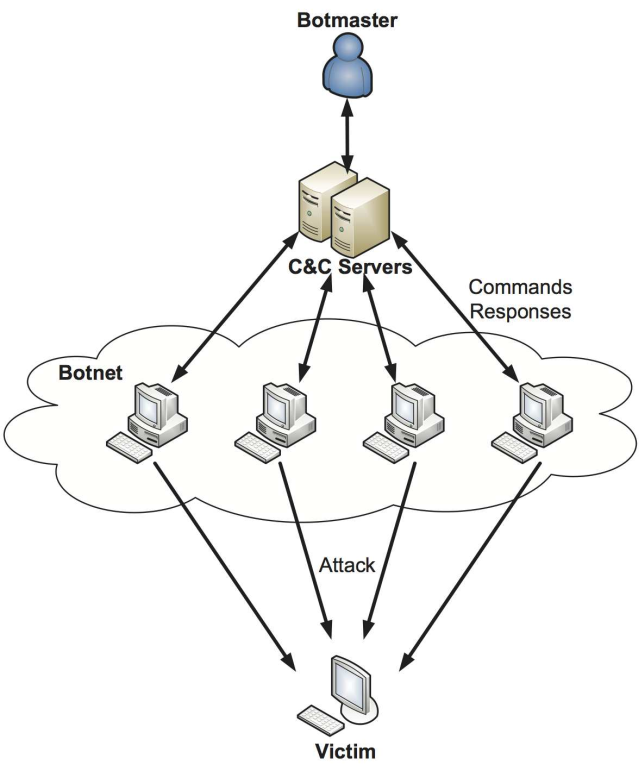
\includegraphics[width=6.8cm]{CentralisedBotnet.png}
    \caption{Centralised botnet architecture \cite{SurveyArchitectures}}
    \label{fig:CentralisedArchitecture}
\end{figure}

\textbf{Decentralised botnets}  This newer architecture of botnets was created to circumvent the singular point of failure, a centralised botnet has. One such variant uses a \emph{DGA} (Domain Generation Algorithm) to generate new domain names given certain environment variables such as the date etc. This allows the botmaster to use different servers to distribute his malware. Sinkholing one such server simply delays the process of malware distribution, but does not kill the botnet \cite{AMP2P}. Another architecture lies in the P2P connected botnets, the focus of this thesis. \\

P2P botnets distribute malware between peers, instead of having them poll the data from centralised servers. This is done by differentiating bots between superpeers, which are routable servers that can directly be contacted, and peers, which are not routable and thus have to poll information from superpeers \cite{AMP2P}. \\

In general each superpeer in a P2P botnet holds a list of neighbours (also superpeers), that can directly be contacted. This \emph{neighbourlist} differs between bots, since it is dynamic and thus changes over time, depending on the accessibility of the neighbours. Each bot runs periodic \emph{MM} (membership maintenance) cycles in order to identify non responsible bots within its neighbourlist. Non responsive bots are often discarded at a given point. This also means that a superpeer will try to gain new neigbhbours, once its neighbourlist reaches a low threshold of entries. This is done by contacting reliable neighbours and polling from their neighbourlist \cite{AMP2P}.

\begin{figure}[H]
    \centering
    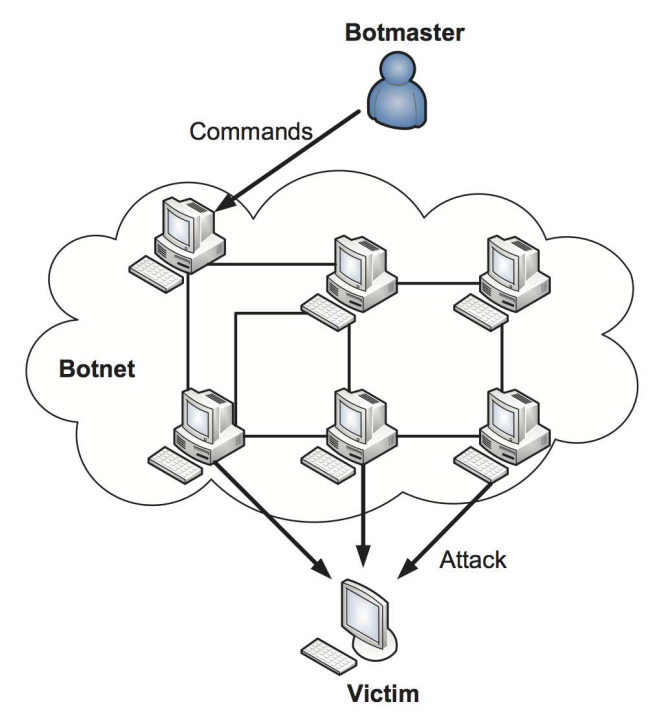
\includegraphics[width=6.8cm]{DecentralisedBotnet.png}
    \caption{P2P botnet architecture \cite{SurveyArchitectures}}
    \label{fig:P2PArchitecture}
\end{figure}

\subsubsection{Crawlers}
\emph{The following subsections provide a brief overview over common crawler characteristics and implementation techniques as well as anti-crawling techniques of botnets} \\

Crawlers are used to retrieve information about a botnets size as well as communication behaviour. A crawler uses the botnet specific communication protocols to contact and communicate with peers. In order to do this, the crawler itself disguises itself as a peer and participates in the botnet. Often, a botnet needs to be reverse engineered to fully understand the protocols needed to insert a sophisticated crawler \cite{kang2009towards}. \\

One fluke of crawlers is the inability to contact peers, that are hidden behind \emph{NAT} (Network Adress Translation), which are not publicly reachable over the internet. These peers often represent the biggest part of a botnets population (up to 90\%) but can only be estimated \cite{AMP2P}.

\subsubsection{Anti-crawling techniques}
Most P2P botnets apply anti-crawling techniques that identify and block crawlers from botnet participation. These can be classified into prevention, detection and response:

\begin{itemize}
    \item \textbf{Prevention}  Botnets can try to prevent crawlers by design. They either stop the crawler from any communication or try to slow it down drastically, often focusing on neighbourlist return mechanism. One example for this is to only return a small portion of a neighbourlist, when a peer receives a neighbourlist request. Some botnets have peers solve time intensive algorithms before receiving a neighbour response \cite{AMP2P}.
    \item \textbf{Detection}  In order to detect unusual behaviour, botnets might blacklist IPs that send many requests in a given time. If the protocol is not implemented in the proper way, a botnet might also detect crawlers by observing communication anomalies, or using botnet intern \emph{sensors} \cite{andriesse2015reliable}.
    \item \textbf{Response}  Often botnets contain static blacklists of IP adresses, that are known to monitor botnets. Alternatively some botnets just start a DDoS attack on the IP monitoring node \cite{AMP2P}.
\end{itemize}

Sality uses prevention by only letting a peer return one random neighbour, whenever it receives a neighbourlist request. In order to circumvent this restriction, a crawler for Sality is able to send neighbourlist requests continously to a peer until it converges towards the set of neighbours \cite{AMP2P}. 

\subsubsection{Sensors} \label{sec:Sensors}
Sensors are passive components injected into the botnet to receive messages without actively having to poll. Sensors are deployed to the network and announce themselves. The goal is to get into as many neighbourlists as possible to be spread even further. Thus in contrast to crawlers they can also reach peers instead of just superpeers, since their information will be propagated by superpeers, that give out reliable neighbours. This leads to regular peers contacting the sensor. Since most botnets, such as Sality evict unresponsive neighbours from neighbourlists, sensors must deploy the botnet specific communication protocols and furthermore react to incoming messages. Thus they are harder to maintain and setup than regular crawlers, but provide deeper insight into the botnet topology while being able to discover all bots not only superpeers. 

\subsubsection{Sality} \label{sec:Sality}
This thesis investigates the P2P version of the botnet Sality, that spreads via a polymorphic file infector for windows executables. Sality originally was developed as a centralised botnet, which was first observed in 2003. In 2008, the first P2P version (V3) was found, followed later on by the newest, most resiliant version: V4 \cite{P2PWNED}. Both V3 and V4 are still active today. \\

\subsection*{Overview} \label{subsec:SalityOverview}
Sality infects machines by concatenating malicious payload to valid windows binaries. Then the entry point of the binary is obscured, such that it executes the malicious code, and afterwards jumps back to the original binary \cite{SP2PVN}. This way, new malware can easily be deployed at any time by letting the malicious binary download new instructions that will be executed. The new included malware can then be used to carry out a number of tasks, such as shutting down services, deleting/encrypting files, sending spam, using the host for computational tasks etc. The propagation of new malware through the Sality botnet is as follows: The malicious code is deployed to certain servers by the botmaster. He then proceeds to distribute a \emph{URL pack} throughout the network, a message of links to the servers that host the new version of the malicious code. This means, that the botmaster can use different IP Adresses each time, since they will be part of the propagated URL pack. Each bot that receives one such pack downloads and executes the new malware \cite{SP2PVN}. This leads to the necessity of URL packs having a unique \emph{sequence number}, since a bot should not download outdated malware. When a new URL pack is released, this number is simply incremented, such that different versions can be discriminated. This necessarily leads to the situation of different URL pack versions being present in a snapshot of the botnet at times, when a new pack has just been released by the botmaster. \\

\subsection*{Protocols} \label{subsec:SalityProtocols}
Salitys superpeers typically hold a neighbourlist of up to 1000 entries, that additionally contains the \emph{LastOnline} timestamp, a \emph{GoodCount}, IP adress, Port and UID for each neighbour. \\

The main message types according to \cite{AMP2P} are:

\begin{itemize}
	\item \textbf{Hello message}  Probes a neighbour for responsiveness. On a successful response, the LastOnline timestamp is set to the current time and the GoodCount is incremented. If a timeout occurs or the bot is unresponsive, the GoodCount is decremented. With the probe message, the current sequence number is also delivered.
	\item \textbf{Neighbourlist request message}  Probes a neighbour for additional superpeers. Bots use this to build their corresponding neighbourlist. The receiving peer will respond with one randomly chosen entry from a list of potential candidates.
\end{itemize}

The MM cycle is invoked every 40 minutes, which starts the following processes for each neighbour sequentially:

\begin{enumerate}
    \item Probe the responsiveness of the neighbour using a hello message.  Depending on the sequence number received, either ask for the whole URL pack, if its sequence number is lower or send back its own URL pack, if it is higher.
    \item The own superpeer status is tested. This is necessary for a bot to know if it is a superpeer and can propagate messages. When a bot is initialized it starts off with UID = 0, meaning its superpeer capabilities are unknown. If it has any other UID it is a superpeer. Thus, a bot with a UID of 0 will test his own status.
    \item If the size of the own neighbourlist is $<$ 980 and the neighbour has a high GoodCount, it is also probed for a neighbour entry. The answering superpeer returns an entry that  is chosen from a list of potential candidates that have a high GoodCount.
\end{enumerate}

After the cycle, a cleanup process takes place. Bots that have a GoodCount less than are dropped from the list, if the size of the neighbourlist is at least 500. \cite{AMP2P}. \\

\subsubsection{Strobo crawler} \label{subsec:StroboCrawler}
Haas et al. \cite{haas2016resilience} created a crawler, that estimates the size and connections of the Sality botnet. The main focus of this crawler lies on accurately tracking neighbourlist changes and node churn of the network via high frequent periodic crawling. Figure \ref{fig:StroboCrawler} dsiplays the basic architecture deployed. It consists of three modules and a list of enumerated nodes that is maintained by the Prober Module.  This list contains all known peers, that are periodically probed by the Prober Module at a given frequency $f_{c}$. The list is further distinguished into all nodes $V^{M}$ and online nodes $V^{O} \subseteq V^{M}$. Incoming messages, such as responses, are handled via the Receiver Module. If the Receiver Module receives a message, it reports it to the Prober Module to update the lists of nodes. If the received message is a neighbourlist message, new unknown nodes are potentially discovered. A Session Module contains online information of nodes in form of sessions. The sessions consist of points of first and last contact. Sessions are kept open, if the bot does not time out. In this case a timeout is defined as not answering a predefined number of probes. If the bot does time out, it is removed from the lists of known nodes.

\begin{figure}[H]
    \centering
    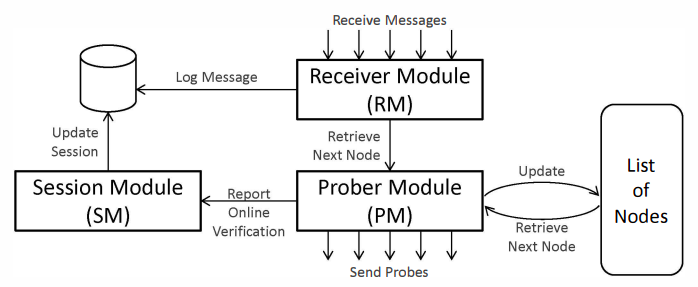
\includegraphics[width=\textwidth]{StroboCrawler.png}
    \caption{Strobo Crawler introduced in \cite{haas2016resilience}}
    \label{fig:StroboCrawler}
\end{figure}

Snapshots of the discovered network architecture can be reconstructed for specific timestamps. A general reconstruction that is valid over an undefined period of time is not possible, because of node churn and MM resulting in a changing network topology. To reconstruct such a topology, Haas et al. \cite{haas2016resilience} explain a time constrainted method. First off, a timestamp $t$ has to be chosen. Then, for each peer the times of the last and next MM cycle around timestep $t$ are determined. This is done, since neighbourlists are not consistent during MM cycles and thus the topology should be reconstructed inbetween such cycles. Since these MM times differ for each bot, the topology is not reconstructed for the specific timestamp $t$ but rather for a $\delta(t)$, where $\delta$ is a function that determines the offset of the time at topology information is collected to the time $t$. \\

The Sality specific implementation of the Strobo Crawler and graph reconstruction uses hello messages for session initiation. Once the online status of a bot has been confirmed, neighbourlist requests are send out. If neighbourlist replies are received by the Receiver Module, hello messages are no longer send \cite{haas2016resilience}. To deduct the MM cycle information, a seperate sensor node is deployed, that receives messages of MM cycle starts. Since Salitys superpeers only share information about specific candidate bots, that have a high GoodCount as explained in \ref{subsec:SalityProtocols}, only these peers can be retrieved. 

\section{Simulation design} \label{System Design}
\emph{This chapter describes the system design of the simulation environment. Firstly a brief overview of the botnet is given. Afterwards the individual entities are explained in detail.} \\

\subsection{Overview}
% Explain generel botnet architecture. Use UML overview.
To test malware propagation strategies, as well as crawlers, a simulation environment in \emph{OMNeT++} (Objective Modular Network Testbed in C++) has been created. OMNeT++ is a discrete event simulation framework. In a discrete event system, state changes happen at specified time instances without delay. The time between events is skipped, since no actions are specified. Events itself such as sending a message are retrieved from an event queue and executed sequentially \cite{vargaOmnet++}. The simulation time is given in seconds. These properties can be used to simulate large periods of real network behaviour within a short period of time, depending on computing power. Thus an implementation via the OMNeT++ framework is very scalable and well suited for simulating potentially big P2P botnets. \\

The simulation environment this thesis describes, features an implementation of Salitys protocols, message formats and superpeer behaviour. Regular peers are of no interest in the simulation, since they cannot propagate URL packs and thus do not supply information about the botmaster. Additionally the behaviour of different crawlers is also implemented.
The main entities of the simulation are:

\begin{itemize}
    \item \textbf{Botmaster}  The botmaster propagating the malware. Three different versions of the botmaster can be selected, that propagate the URL packs in different ways, further explained in \ref{subsec:DistributionMethods}.
    \item \textbf{Superpeer}  The public routable peers of the botnet, that have been crawled in the existing network and parsed into the simulation environment as visualized in \ref{subsec:StroboCrawler}. These superpeers behave conform to the Sality protocol explained in \ref{subsec:SalityProtocols}.
    \item \textbf{Crawler}  The crawler to traverse the botnet towards the botmaster. Multiple crawler versions can be selected, each using different algorithms to explore the network that are further reviewed in \ref{subsec:CrawlerVersions}.
\end{itemize}

All these entities are defined as modules. OMNeT++ modules declare the individual nodes of the simulated network. These are able to communicate with each other and execute arbitrary behaviour, since they are simply written in C++. This means that the botmasters, superpeers and crawlers each are defined in C++ classes with their own individual behaviour. To declare modules, a module description, as well as behaviour have to be implemented. The description is in form of a NED file, which defines parameters, as well as communication gates. Figure \ref{fig:BotmasterNED} displays an example setup of a botmaster module. The parameters can be accessed in the C++ classes, that implement the behaviour. Gates determine ways for other modules to communicate with a specific module. \\

\begin{figure}[H]
    \centering
    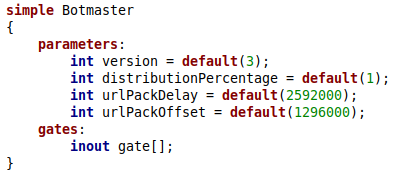
\includegraphics[width=8cm]{BotmasterNED.png}
    \caption{Example NED file of a botmaster}
    \label{fig:BotmasterNED}
\end{figure}

Modules are able to communicate via messages. In OMNeT++ messages come in the form of the cMessage class, that can be transmitted between modules. These messages hold different attributes as well as network statistics such as a message name, creation time, sender, receiver, transmission channel etc.. The cMessage class can be extended to create individual messages. In the case of this thesis, it was extended to create URL pack messages. As described in \ref{subsec:SalityProtocols} messages between superpeers are exchanged in different states. Firstly, with each MM cycle, a peer probes all of its neighbours. This is implemented via a URL probe message. Secondly, if any peer receives a probe message with a lower sequence number than its own, it sends back its sequence number via a URL pack message. When it receives a higher sequence number, it asks for the whole URL pack via its own probe message. Since regular peers are of no interest in this thesis, the superpeer probe message is not implemented. This however does not change superpeer behaviour and thus can be omitted without altering simulation output. Figure \ref{fig:SalityMessageFlow} displays the basic superpeer behaviour on receiving a message. \\

\begin{figure}[H]
    \centering
    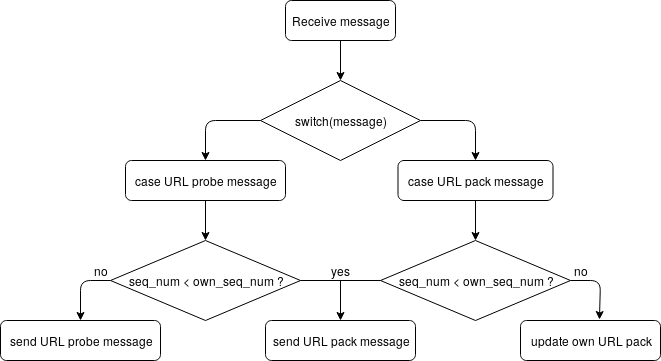
\includegraphics[width=\textwidth]{pictures/SalityMessageFlow.png}
    \caption{Superpeer behaviour on receiving a message}
    \label{fig:SalityMessageFlow}
\end{figure}

All communication happens via channels. OMNeT++ channels represent connections between modules. Channels can define behaviour such as network delay etc.. In order to simulate global communication behaviour, a minimum delay of 50ms is assumed. Furthermore delay is added for each individual message transmission based on a geometric distribution. This distribution was found out to fit existing network behaviour very well. \\

To condense network setup information, OMNeT++ also uses NED files. These network specific files contain modules, channels, connections and further information on the network architecture.
Figure \ref{fig:SalityNED} displays an example NED file of the botnet Sality. For brevity information like imports etc. is skipped. Also only a few superpeers and connections are included. The network sality contains a channel definition, submodules and connections. The channel is used for the communication between the individual modules and holds the described default message delay of 50ms. The submodules contain the set of superpeers, a crawler and a botmaster module. The crawler is optional and only used for the crawler evaluation in \ref{sec:Crawlers}. The set of peers and the botmaster however are needed for the simulation of the Sality network. Each module is further connected to other modules in the connection section. In this case bidirectional channels are used, since superpeers need to be able to respond to URL pack messages. \\

\begin{figure}[H]
    \centering
    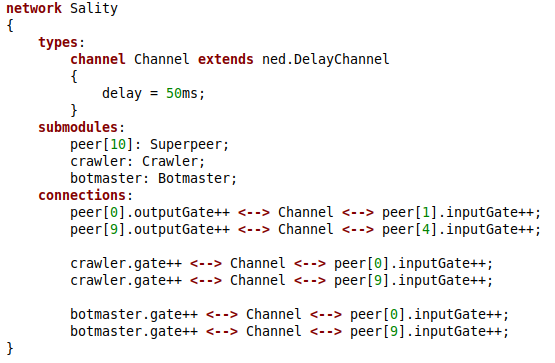
\includegraphics[width=10cm]{SalityNED.png}
    \caption{Simplified Sality NED file}
    \label{fig:SalityNED}
\end{figure}

Since snapshots of the Sality botnet are static, the simulation environment also holds a static set of superpeers. For the evaluation of botmaster strategies \ref{sec:BotmasterStrategies} the propagation is tested in this static environment. However, since crawlers in existing botnets need to overcome node churn, superpeers in the simulation also implement node churn behaviour. This is then used in \ref{sec:Crawlers} to better simulate real crawling behaviour. \\

\subsection{Steps}
To run a simulation of the Sality botnet, first off the network topology has to be established. For this task, the output of the Strobo crawler \ref{fig:StroboCrawler} is used to reconstruct the network structure, which is saved in a graphml file. This file declares nodes and edges. Each node represents one superpeer, each edge a connection between two superpeers of the existing Sality network. \\

\begin{figure}[H]
    \centering
    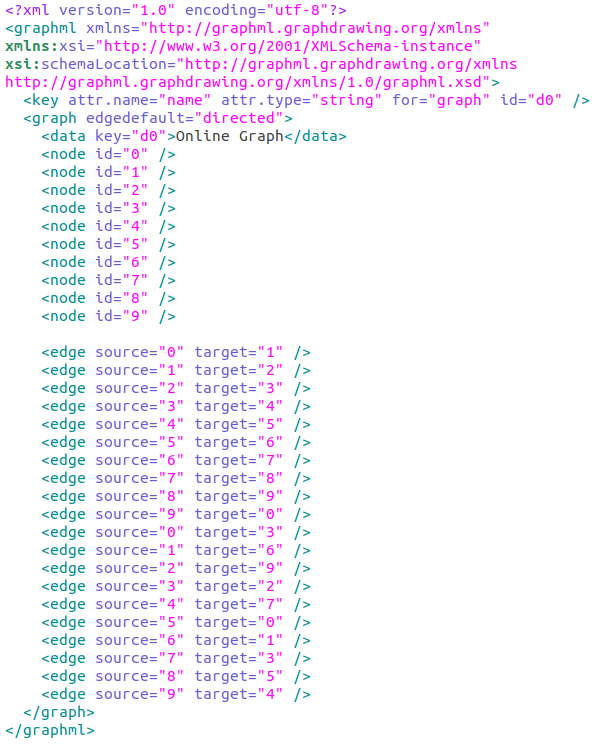
\includegraphics[width=10cm]{GraphmlExample.png}
    \caption{Simplified graphml file with 10 nodes and 20 connections}
    \label{fig:SimplifiedGraphml}
\end{figure}

These graphml files are used to create the simulation environment, which is a parsed version of the connection graph. Thus, each node of the graphml file represents one superpeer entity in the OMNeT++ simulation, each edge a connection between two superpeers. A script (graphml-to-ned.py) parses the GraphML file and returns a NED file that can be used in OMNeT++. This script additionaly introduces a botmaster to the topology and optionally a crawler. \\

Once a network structure has been established, different simulations can be run depending on the botmaster strategy and crawler version of interest. This is done using a shell script (runSimulation.sh) and supplying the wanted version as the first argument. Versions are of the following format: V\{\emph{number}\}, where \emph{number} denotes the simulation to be run. More information about the run files and simulation to number mappings can be found in the projects READMEs. \\

In order to evaluate the resulting run data, it is written to log files during the simulation process. This provides the groundwork for further processing of the information in order to retrieve insights on propagation statistics and crawler results. Different scripts have been written to further analyze botmaster and crawler behaviour.

\section{Evaluation}

\subsection{Botmaster strategies} \label{sec:BotmasterStrategies}
\emph{This section evaluates the different strategies the botmaster potentially uses to distribute URL packs. The botmaster strategy is estimated by comparing statistics from the simulation environment to ones from Sality. In order to achieve this, the simulation is run with different hyperparameters to account for various botmaster behaviours. Each simulation run logs relevant statistics. The Strobo Crawler \ref{subsec:StroboCrawler} provides log files from the Sality network. These files are then further analyzed and compared to find a propagation technique that fits the real behaviour.}

\subsubsection{Distribution methods} \label{subsec:DistributionMethods}
The following distribution methods of a botmaster behaviour are evaluated:

\begin{enumerate}
    \item Active Botmaster 1 (AB1): This botmaster is not part of the network. Instead, it pushes the new sequence numbers to a set of superpeers, using the default communication protocol described in section \ref{subsec:SalityProtocols}.
    \item Active Botmaster 2 (AB2): Also not part of the network. This variant pushes the new URL packs directly to a set of superpeers, avoiding the default communication protocol, resulting in faster propagation time compared to the Active Botmaster 1. This method could possibly be used in the existing Sality botnet, given the communication patterns described in \cite{AMP2P}.
    \item Passive Botmaster (PB): This botmaster is part of the network in form of controlled superpeers. These controlled peers simply increment their own sequence numbers periodically without the need to actively push it to a set of superpeers. This means, that other superpeers have to actively poll the new URL packs. Essentially this is equivalent to an AB2 without message delay or loss, since no network communication between the botmaster and the controlled peers play a role. However, since the botmaster has to own the superpeers, the amount of controlled peers is realistically limited. Furthermore he would not be able to simultaneously update all controlled peers without delay. Because of this, the PB is only tested with the botmaster as part of the network but no further controlled superpeers, since this is already done in AB2.
\end{enumerate}

In additon to the distribution methods, the active botmaster is also able to choose the set of superpeers he distributes the URL pack towards. Different $peer\_selection$ strategies are explored: 

\begin{itemize}
    \item \textbf{Random selection}  As the name suggests, the botmaster chooses a random subset of superpeers to propagate the malware towards. In the simulation this is accounted for by choosing an evenly distributed subset of superpeers amongst all bots. 
    \item \textbf{Most neighbours}  The botmaster could achieve faster propagation time by contacting superpeers with a high neighbour count. If the botmaster actively monitors his own botnet, he is able to estimate neighbourhood information similar to the Strobo crawler explained in \ref{subsec:StroboCrawler}.
    \item \textbf{Next MM cycle}  Another valid strategy is to choose bots, that enter their respective MM cycles earliest according to the current timestep. This provides faster propagation, since these superpeers contact all their neighbours within the next cycle, directly sending the new URL pack.
\end{itemize}

\subsubsection{Evaluation parameters}
To provide a meaningful comparison, different distribution parameters are evaluated. Each strategy is thus evaluated for a set of different hyperparameters:

\begin{itemize}
    \item $sim\_time\_limit$: The simulation time limit in seconds. This is mainly used to get different propagation behaviour since MM-cycles play out differently depending on the time of the simulation.
    \item $distribution\_percentage$: If the botmaster is using one of the above mentioned active distribution methods, this percentage states the amount of peers he directly contacts.
\end{itemize}

Due to the different hyperparameter combinations, individual simulations are run with the following parameter sets: \\

\begin{itemize}
    \item Passive botmaster: In this case only $sim\_time\_limit$ = \{15768000s, 31536000s\} holds different values. No further hyperparameters are evaluated.
    \item Active botmasters: $sim\_time\_limit$ = \{15768000s, 31536000s\}, $distribution\_percentage$ = \{10, 20, 30, 40, 50\}. Both active botmaster distribution methods are evaluated as the crossproduct of the $sim\_time\_limit$ and $distribution\_percentage$, resulting in 10 different simulations each. The distribution percentages were evaluated via a trial and error approach to find a best fit to the botnet data.
\end{itemize}

In order to retrieve meaningful statistics given certain hyperparameter settings, each simulation is run multiple times with different seeds. This affects the random propagation and release times of URL packs, such that each run yields different results. When also considering the different $peer\_selection$ strategies, this results in a total of $3 \times (3 \times (10 + 10) + 1) = 183$ runs. This number is sufficient to gather average distribution statistics. The following run statistics are evaluated:

\begin{itemize}
    \item $mean\_propagation\_delay$ in seconds until $x\%$ superpeers receive a URL pack, calculated by: $$\frac{1}{n} \times \sum_{i=1}^{n}(receive_{i}^{(x)} - release_{i})$$ where $receive_{i}^{(x)}$ is the timestamp in seconds, at which $x\%$ superpeers received URL pack of sequence number $i$ and $release_{i}$ the number timestamp in seconds, at which the botmaster released the URL pack of version $i$.
    \item $max\_pack\_delay$: Max propagation time in seconds until $x\%$ superpeers receive a URL pack. This is the maximum amount of seconds measured, until any URL pack was propagated by $x\%$.
    \item $min\_pack\_delay$: Min propagation time in seconds until $x\%$ superpeers receive a URL pack. This is the minimum amount of seconds measured, until any URL pack was propagated by $x\%$.
    \item $message\_loss$, calculated by: $$\frac{1}{n} \times \sum_{i=1}^{n}(numPeers - numPeers_{i})$$ where $numPeers$ is the total number of superpeers in the network and $numPeers_{i}$ the number of superpeers, that have received the URL pack of version $i$.
\end{itemize}

In order to retrieve meaningful results, the statistics of the individual runs are collected. Afterwards the mean values for the same runs with different seeds are taken to remove outliers and gather meaningful insights. \\

To be able to compare the simulation results to the real Sality behaviour, multiple message logs from the Strobo Crawler \ref{subsec:StroboCrawler} have been gathered. These logs are in the form of messages, that the Receiver Module collected from peers. Each message holds the following information:

\begin{itemize}
    \item \textbf{Timestamp}  The time at which the Receiver Module received the message in the format: JJJJ-MM-DD hh:mm:ss.
    \item \textbf{IP}  The IP address of the peer.
    \item \textbf{NodeType}  The type of the peer. A 'client' denotes a peer that initiated the request and thus can either be a regular peer or a superpeer. A 'server' denotes, that the received message is a response to a message of the Prober Module and thus comes from a superpeer.
    \item \textbf{CMD}  The protocol \ref{subsec:SalityProtocols} used by the contacting peer. 
    \item \textbf{PackID}  The sequence number of the URL pack the peer holds.
\end{itemize}

To evaluate the URL pack distribution time over the superpeers, only messages with the CMD of 'server' are evaluated. For all messages of these superpeers, that have been received, the message with the earliest timestamp is considered to be the time of the superpeer receiving the URL pack for the first time. Of course this is not conform to the real reception time, since there is always a delay $\delta_{i}$ for each superpeer message reception $rm_{i}$ of the Receiver Module. This $\delta$ is defined by: $rm_{i} - recep_{i}$, where $recep_{i}$ denotes the time at which superpeer $i$ received the URL pack for the first time from another superpeer $j$.

\subsubsection{Results} \label{subsec:distrMethodsResults}
Both in the real Sality network and the simulation all URL packs are eventually propagated, without one being missed out by certain peers, which results in a $message\_loss = 0$ for all simulation runs. This indicates that the superpeers form a fully connected graph, such that all messages eventually are propagated to all peers. Haas et al. \cite{haas2016resilience} also pointed out, that the Sality botnet is rather dense. Peers either know most other superpeers, or nearly none if they just joined. This is probably a result of the long intervals between MM cycles. \\

Figure \ref{fig:PBstats} displays the propagation statistics for the passive approach. The data does not fit Salitys statistics very well, especially the average/maximum URL pack delay are off. However, on the minimum delay, a drastic jump is visible from $5-60\%$ distribution percentage that is probably due to the simultaneous overlapping MM cycles of multiple superpeers. This result suggests, that the botmaster is not just part of the network, but rather uses a different distribution mechanism. This makes sense, since the P2P structure of Sality would not efficiently be used, if the botmaster itself was part of it. It would lead to the botmaster being the C2 server, which could simply be traced and sinkholed. Thus, the passive botmaster does not seem to be the strategy followed. The following sections display and interpret the results of the different $peer\_selection$ stategies for the active botmasters.

\begin{figure}[H]
    \centering
    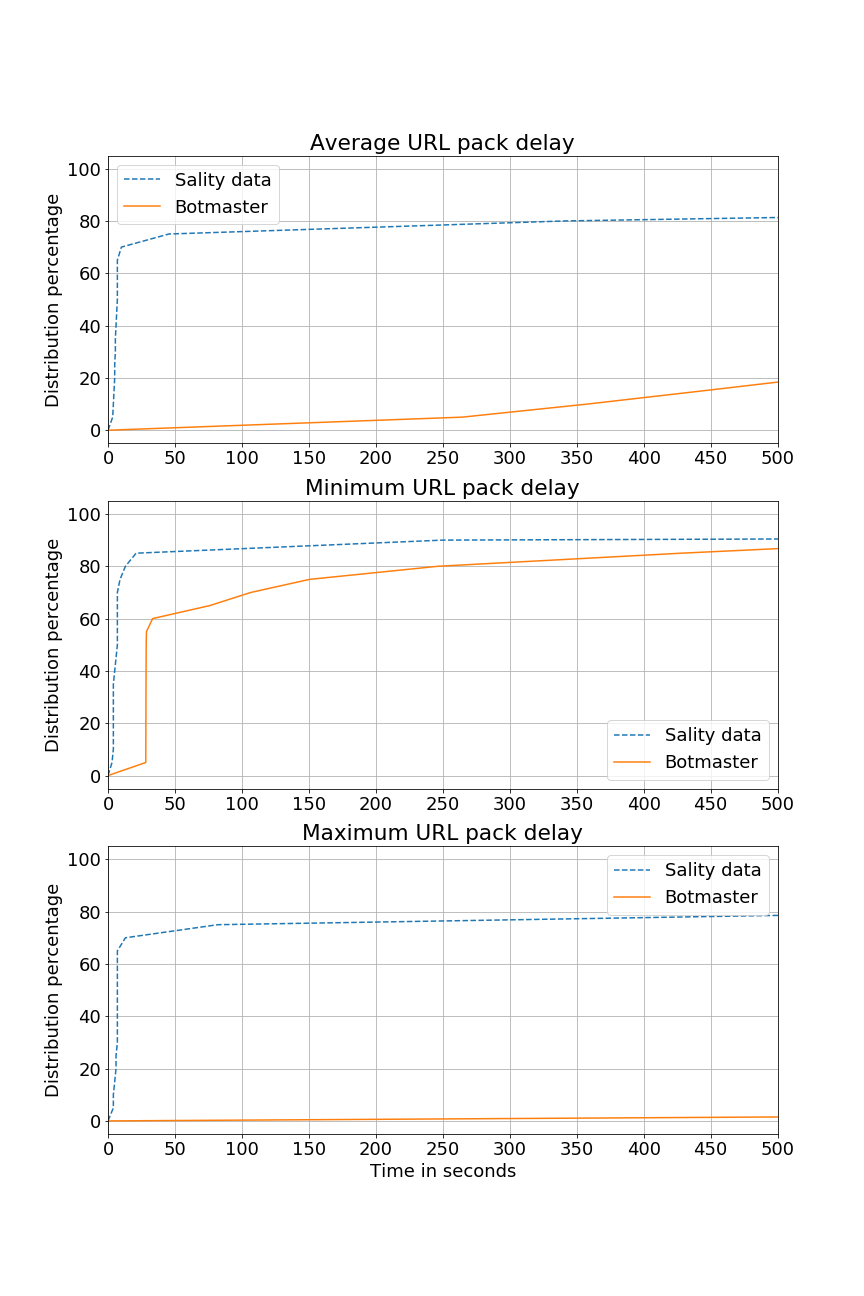
\includegraphics[width=\textwidth]{BV1-PS1.png}
    \caption{Distribution statistics of the PB}
    \label{fig:PBstats}
\end{figure}

\subsubsection*{Random selection}
The figure \ref{fig:AB2-PS1stats} shows the statistics for the AB2 method with different values for $distribution\_percentage$. These curves approximate the real data very well. Especially the minimum URL pack delay seems to follow Salitys distribution statistics for nearly all different distribution percentages. It is noteworthy, that in the Sality network approximately $70\%$ o the superpeers receive the new malware in less than a minute. Afterwards the time towards $100\%$ propagation rises exponentially. This could be due to the above referenced Sality density and connection attributes. The closely connected superpeers probably propagate the according packs towards each other, since each established one will receive multiple messages from other superpeers once a pack has been released. The newer outlier peers however often have to wait multiple MM cycles to receive the new pack. This could mean, that the Sality network consists of approximately $70\%$ closely connected and $30\%$ outlier superpeers. This leaves the question on how many peers the botmaster directly contacts to propagate the new malware. According to the average URL pack delay, the $30\%$ curve seems to fit very well. This could likely be the case if the botmaster itself utilizes a botnet monitoring mechanism to follow node churn. 

\begin{figure}[H]
    \centering
    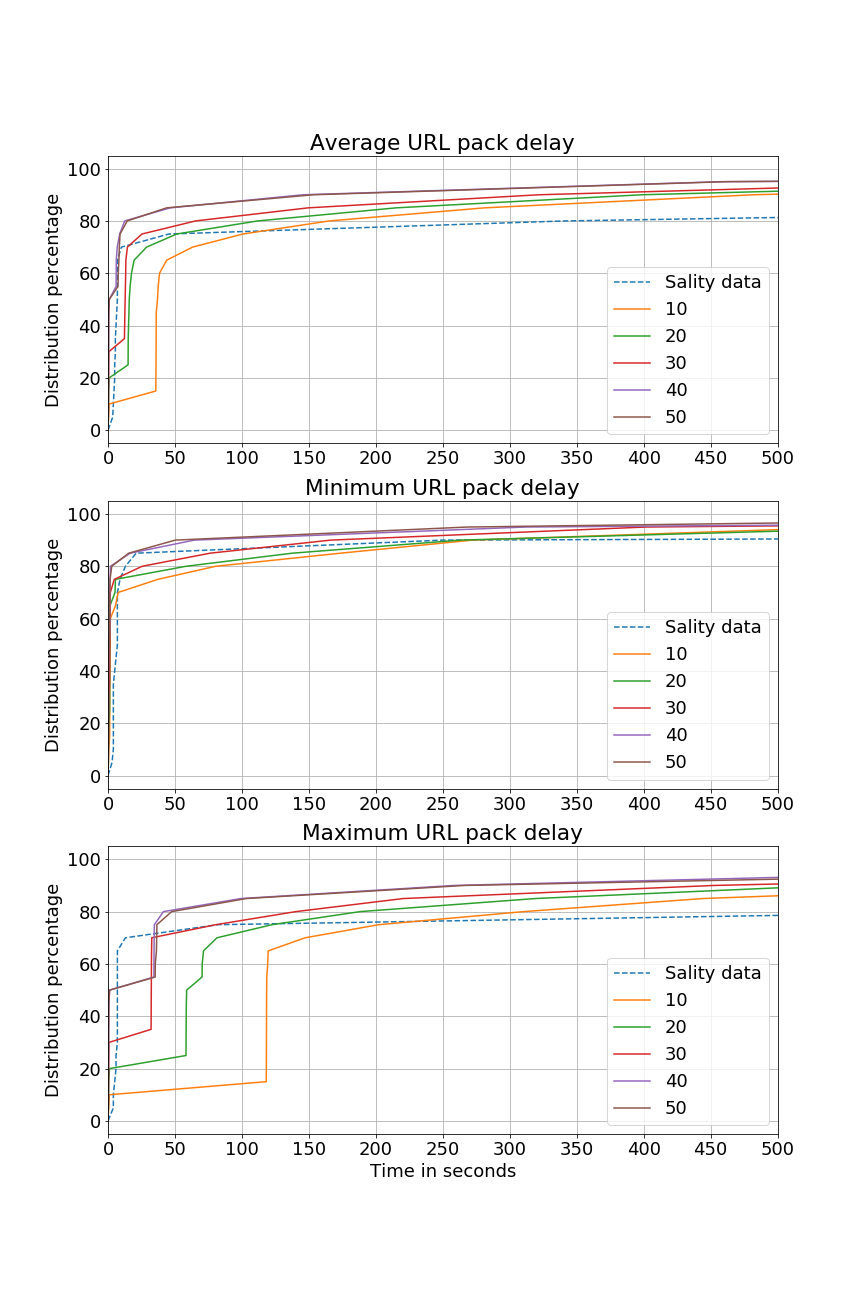
\includegraphics[width=\textwidth]{BV3-PS1.png}
    \caption{AB2 selecting peers randomly}
    \label{fig:AB2-PS1stats}
\end{figure}

The AB1 distribution mechanism \ref{fig:AB1-PS1stats} does not differentiate from the AB2 a lot. The statistics are nearly identical. This is due to the fact, that the message propagation delay is only a fraction $\approx 0.008\%$ of the MM cycle delay. This results in the MM cycle delay being way more influential on the message propagation than communication overhead of the protocol. Thus, for the evaluation of the remaining $peer\_selection$ strategies only the AB3 approach is used. This is because after evaluation of the different strategies, the delay due to the communication protocol does not influence the output of any $peer\_selection$ strategy in a relevant way.

\begin{figure}[H]
    \centering
    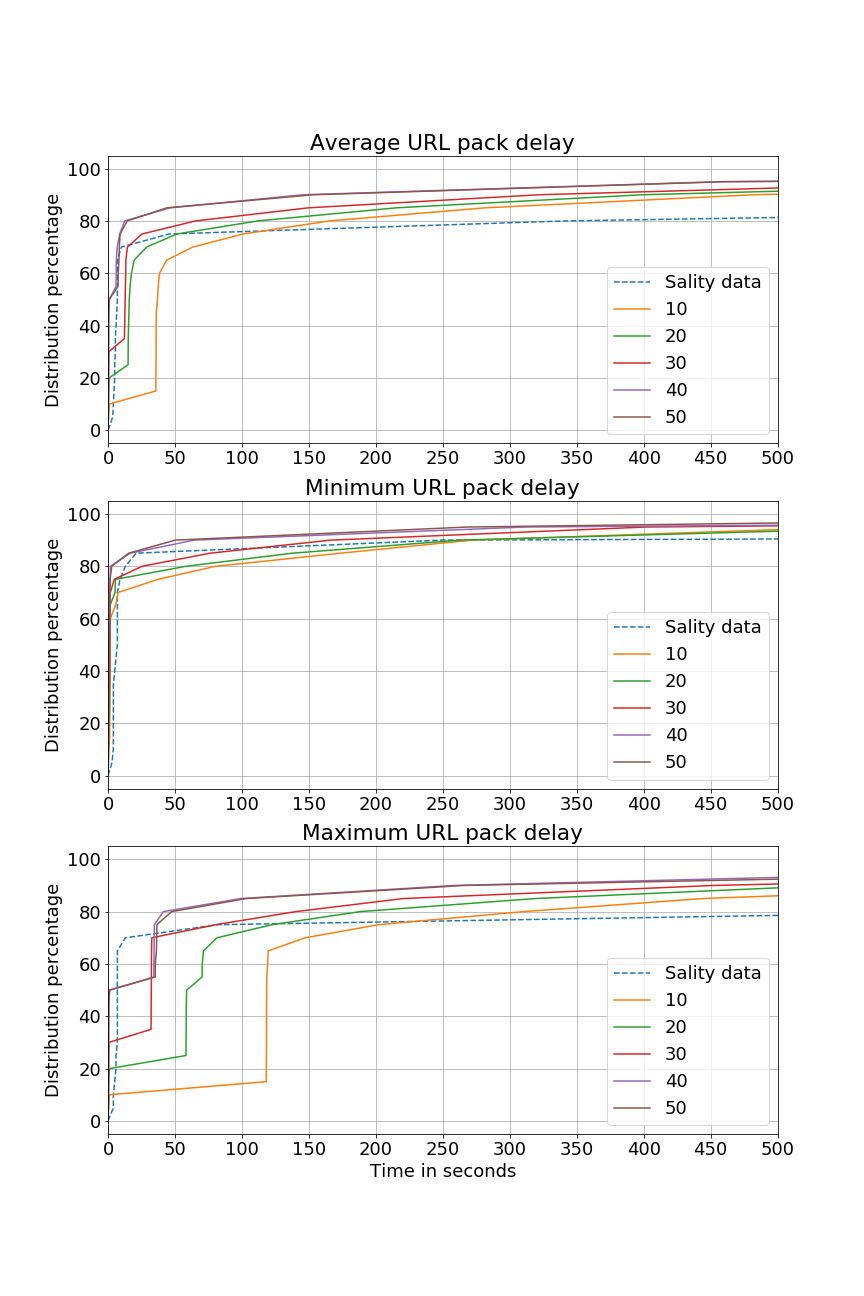
\includegraphics[width=\textwidth]{BV2-PS1.png}
    \caption{AB1 selecting peers randomly}
    \label{fig:AB1-PS1stats}
\end{figure}

\subsubsection*{Selection based on the neighbourlists}
Figure \ref{fig:AB2-PS2stats} displays the evaluation of the neighbourlist $peer\_selection$ strategy. Outstanding similarity can be seen in the minimum URL pack delay, where every $distribution\_percentage$ aligns close to Salitys statistics. 

\begin{figure}[H]
    \centering
    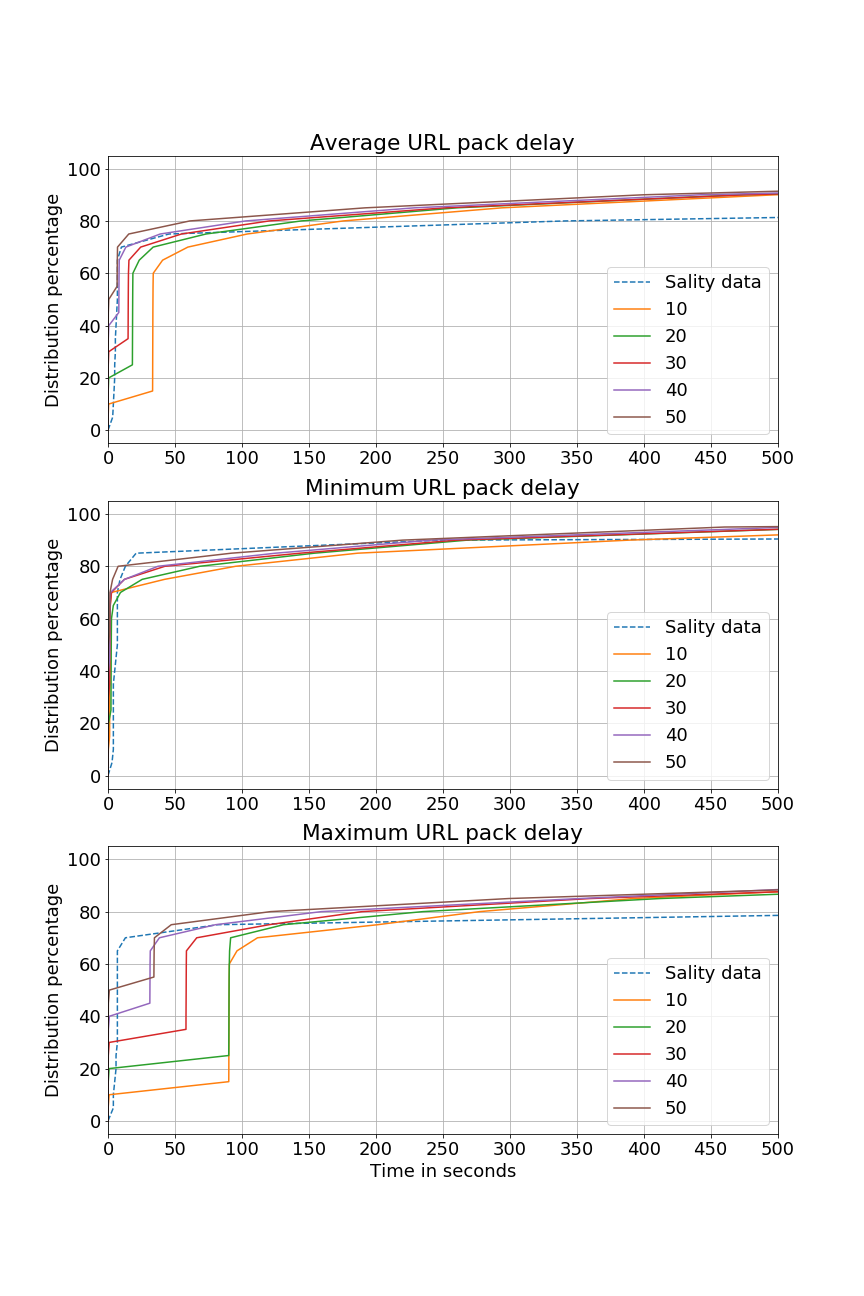
\includegraphics[width=\textwidth]{BV3-PS2.png}
    \caption{AB3 selecting peers based on the neighbourlists}
    \label{fig:AB2-PS2stats}
\end{figure}

\subsubsection*{Selection based on the next MM cycle}

\begin{figure}[H]
    \centering
    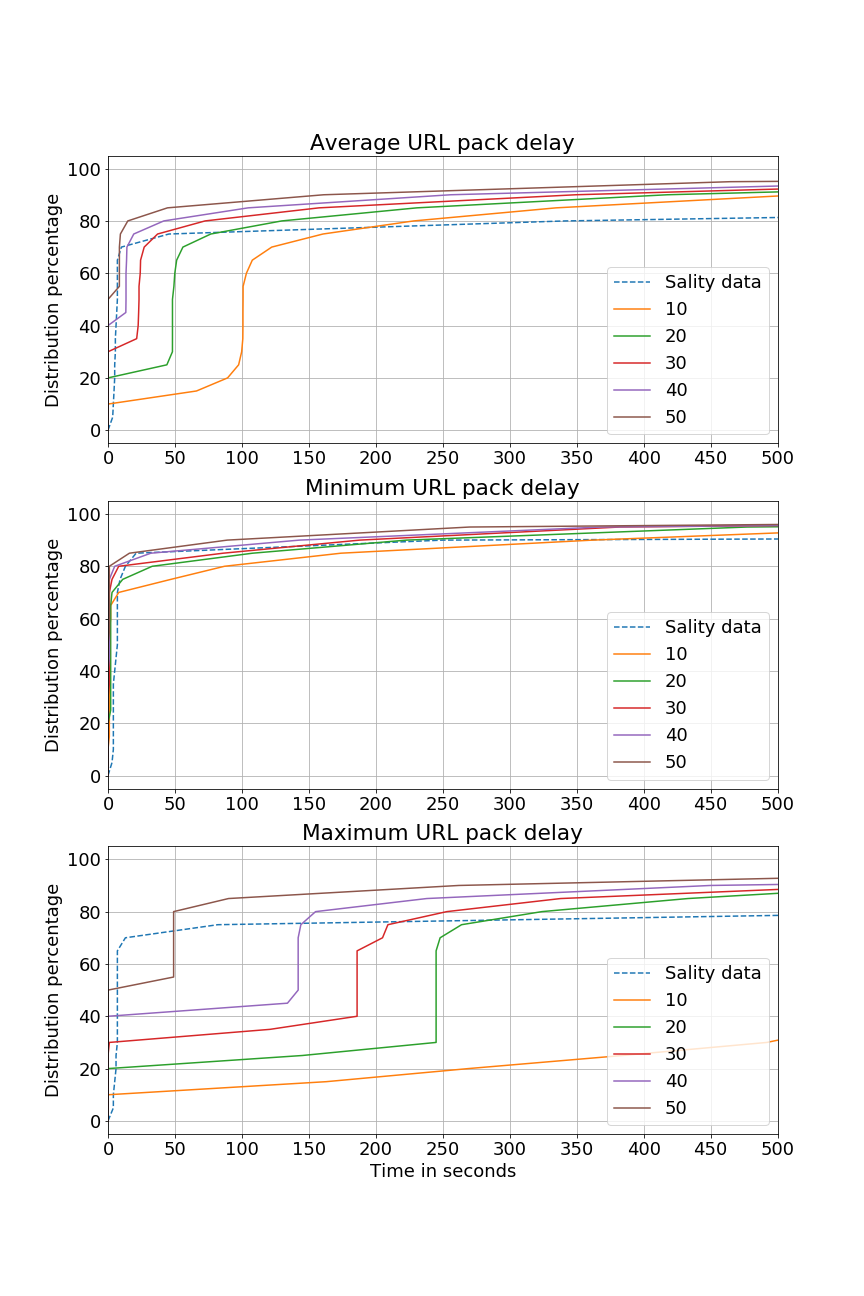
\includegraphics[width=\textwidth]{BV3-PS3.png}
    \caption{AB3 selecting peers based on the MM cycle}
    \label{fig:AB2-PS3stats}
\end{figure}

After evaluating the different botmaster strategies, the AB1 and AB2 methods seem to fit the real data well????. The communication overhead of following Salitys communication protocol does not seem to influence the message propagation in a relevant way. The PB approach is not likely to be used in the real botnet. This is not only due to the unfitting data, but also the drawbacks of being part of the network. For further evaluation of the crawlers, the AB2???? approach is used, since it seems to be the most likely one to be deployed by the real botmaster. Furthermore, crawlers are tested on $20-40\%$ $distribution\_percentage$. To account for node churn and a botmaster that utilizes monitoring techniques for a quickly changing networks, only $10\%$ of the known peers are held constant, whereas the others are randomly changing over time.

\subsection{Crawlers} \label{sec:Crawlers}
\emph{This section evaluates different crawlers that traverse the network towards the malware source, using the distribution method found in \ref{subsec:distrMethodsResults}.}

\subsubsection*{Notation}
For easier comparison between crawlers, a formal model of the botnet is used. Following is a description of all relevant parts: 

\begin{itemize}
	\item  \textbf{$V_{S}$}  The set of all superpeers in the whole botnet.
	\item  \textbf{$V_{E}$}  The resulting set of superpeers, that a crawler outputs. This set contains all superpeers that have been found are potentially connected to the botmaster. $V_{E} \subseteq V_{S}$ thus is a necessary condition.
	 \item  \textbf{$seq_{max}$}  The maximum sequence number of any URL pack that has been propagated by the botmaster.
	 \item  \textbf{$seq_{u}$}  The maximum sequence number of the URL pack bot $u \in V_{S}$ holds.
\end{itemize}

\subsubsection{Crawler versions} \label{subsec:CrawlerVersions}
The following different crawler versions are compared:

\begin{itemize}
    \item \textbf{Crawler V1}  This version holds a mapping of $V_{E}^{(u)} \rightarrow seq_{u}$, where $u$ is the neighbouring bot that is potentially connected to the botmaster. Thus it  saves for each eligible bot the corresponding sequence number in $V_{Eu}$.  $V_{Eu}$ is initially set to all known peers, with each having a sequence number of 1. The peer filtering happens by constantly iterating over $V_{Eu}$, kicking bots that do not hold $seq_{max}$. It does this by sending a URL probe message as explained in \ref{System Design} at timestamp $t_{i}$, where $i$ is the number of the iteration. For each response, it saves the corresponding mapping in $V_{Eu}$. If superpeers do not answer after a time period of $\delta$ has passed, they are probed again $n$ times. If they have not answered after the $nth$ message, they are assumed to be offline and kicked from $V_{Eu}$. Thus, one probing cycle takes at maximum $n \times \delta$ seconds. All remaining superpeers are now compared. Every bot that does not hold the current $seq_{max}$ is also kicked from $V_{Eu}$. This process is repeated until no changes in $V_{Eu}$ happen for $x$ cycles. Figure \ref{CrawlerV1Alg} displays the corresponding algorithm. It is noteworthy, that $V_{Eu}$ has to be iterated two times in order to drop all failing superpeers. In the first iteration $seq_{max}$ ist found over all bots, already dropping ones that have a lower sequence number. In the second one, all peers $u$ with $seq_{u} < seq_{max}$ are dropped. Overall, the time complexity of this algorithm is in $O(n \times (2 + \delta))$, which is feasable, since Sality usually contains less than 1000 superpeers.
    
    \item \textbf{Crawler V2}  This crawler utilizes timestamps and neighbour information in order to filter out superpeers. 
    
    % All bots in $V_{E} \setminus  u$ will be polled for their sequence number again and discarded, if it is less than $seq_{u}$. Periodically sequence numbers between bots in $V_{E}$ will also be compared, and the set accordingly maintained to only hold superpeers with the current $seq_{max}$. This algorithm will probably work well, if the botmaster only has a single entry point.
    % \item Permanently saving bots, that once were in a set of $V_{E}$, when $V_{E} / V_{S} \leq x\%$: Since a botmaster could have multiple entry points, it is necessary to not only consider bots that currently have a high sequence number. Once a converging set has been found, it should be saved as $V_{E_Final}$. Even if the botmaster now entries at a different point, these superpeers will not be lost. Based on the locality of bots in $V_{E_Final}$, different entry points can be estimated.
    % \item Adding another set to save bots, that frequently had a high sequence number: This approach is similar to 2., with the exception, that $V_{E_Final}$ can now also discard entries. A second set $V_{E_Past}$ will be added to hold bots that in the past were in the top $x \%$ of $V_{E}$ based on sequence numbers and timestamps. A good value for $x$ will have to be estimated/learned. Also a score for each bot could be determined. Then, once a bot $u \in V_{E_Past}$ holds $seq_{max}$ again at a given time $t$, it will be considered to be in $V_{E_Final}$. $V_{E_Final}$ can also be a set of a maximum size. Then the superpeer score would be necessary to determine the closest fits.
    % \item Using timestamps: The timestamps at which the superpeers received the new URL pack will also be considered. This approach will use the above algorithms (3. already uses timestamps), but also try to weight superpeers by timestamp. A bot that received a URL pack at an earlier timestamp will be considered closer to the origin.
    % \item Other metrics found during the implementation and testing of the crawler will be included. Especially for fluctuation of bots further methods will probably have to be considered.
\end{itemize}

\begin{figure}[H]  \label{CrawlerV1Alg} 
\begin{algorithmic}
\State $count \gets 0$
\While {$count < x$}
	\State $count \gets count + 1$
	\For {$v \ in \ V_{Eu}$} 
		\State $pollUntilResponseOrTimeout(v)$
	\EndFor
	\State $currentMax \gets 1$
	\For {$v \ in \ V_{Eu}$} 
		\If {$seq_{u} \geq currentMax$} 
			\State $currentMax = seq_{u}$
		\Else
			\State $V_{Eu}.drop(u)$
			\State $count \gets 0$
		\EndIf
	\EndFor
	\For {$v \ in \ V_{Eu}$} 
		\If {$not \ seq_{u} = currentMax$} 
			\State $V_{Eu}.drop(u)$
			\State $count \gets 0$
		\EndIf
	\EndFor
\EndWhile
\end{algorithmic}
\caption{Algorithm of the Crawler V1}
\end{figure}
\subsubsection{Evaluation parameters}
Different metrics are established to measure the success of the crawlers:

\begin{enumerate}
	\item Size of subset $V_{E} \subset V_{S}$ of superpeers potentially connected to the botmaster. The smaller this size, the better the crawler.
	\item Average steps of a superpeer $p$ for $p \in V_{E}$ to the initial superpeer that received the package. The higher this metric, the worse the crawler performed.
	\item Number/percentage of superpeers $p$ for $p \in V_{S}, p \notin V_{E}$ that are closer to the initial source as stated in 2.. This is the amount of superpeers that have not been found, but are potentially connected to the botmaster.
\end{enumerate}

\subsubsection{Results}

\subsection{Summary}

\section{Conclusion}

\subsection{Results}

\subsection{Future work}

\newpage

\section*{Bibliography}
\addcontentsline{toc}{section}{Bibliography}

\nocite{*}
\bibliographystyle{ieeetr}
\bibliography{bibliography.bib}

\section*{List of figures}
\addcontentsline{toc}{section}{List of figures}

\section*{List of tables}
\addcontentsline{toc}{section}{List of tables}

\section*{Acronyms}
\addcontentsline{toc}{section}{Acronyms}
\textbf{P2P} Peer to Peer \\

\textbf{C2} Command \& Control \\

\textbf{DDoS} Distributed Denial of Service \\

\textbf{DGA} Domain Generation Algorithm \\

\textbf{MM} Membership Maintenance \\

\textbf{NAT} Network Adress Translation \\

\textbf{OMNeT++}  Objective Modular Network Testbed in C++) \\

\section*{Glossary}
\addcontentsline{toc}{section}{Glossary}
\textbf{Botmaster} Person in control of the botnet. Can propagate malware throughout the network to be executed. \\

\textbf{Botnet} Set of compromised machines connected to the internet. These computers carry out malicious commands from the botmaster. \\

\textbf{Bot} Infected machine and part of the botnet, that carries out attacks of the botmaster. \\

\textbf{Peer} Synonym to bot. \\

\textbf{Crawler} Entities that traverse the botnet in order to discover bots.\\

\textbf{Sinkholing} Redirecting traffic over a controlled server. \\

\textbf{Entry Point} Superpeers, that the botmaster contacts in order to distribute new malware in a P2P botnet. \\

\textbf{Superpeer} A bot in a P2P botnet, that is routable and can thus exchange neighbourlist information. \\

\textbf{Neighbourlist} A list each superpeer in a P2P botnet owns. It contains information about other superpeers that can be contacted. \\

\textbf{URL pack} A message spread by the botmaster in the Sality botnet. It contains links to servers that hold new malware for the bots to execute. \\

\textbf{Sequence number} The number uniquely identifying a URL pack version. \\

\textbf{LastOnline} The timestamp for a neighbour in a neighbourlist of a bot in the botnet Sality, that states when the neighbour was successfully probed the last time. \\

\textbf{GoodCount} A value for a neighbour in a neighbourlist of a bot in the botnet Sality, that states how reliable the neighbour is. This depends on how many succesfull responses he has given. \\

\textbf{Sensor} A peer of a botnet that evaluates the network traffic and peer behaviour. The goal is to make the IP of a sensor known to all peers, such that the whole communication can be analyzed. \\

\textbf{Node churn} The rate at which peers join or leave the botnet. If this rate is high, the network infrastructure changes often.

\section*{Source code}
\addcontentsline{toc}{section}{Source code}

\end{document}
